\documentclass{article} % For LaTeX2e
\usepackage{nips14submit_e,times}
\usepackage{hyperref}
\usepackage{url}
\usepackage[utf8]{inputenc}
\usepackage{amsmath}
\usepackage[numbers,sort]{natbib}
\usepackage{graphicx}
\usepackage[export]{adjustbox}
\usepackage{footmisc}
\DeclareGraphicsExtensions{.pdf,.png,.jpg,.eps}

%\documentstyle[nips14submit_09,times,art10]{article} % For LaTeX 2.09         



\author{
Gabriel C-Parent\\
Département d’informatique et recherche opérationnelle\\
Université de Montréal\\
\texttt{gabriel.c-parent@umontreal.ca} \\
\And
Dora Fugère \\
Département de mathématiques et de statistique \\
Université de Montréal\\
\texttt{dora.fugere@umontreal.ca} \\
}


\newcommand{\fix}{\marginpar{FIX}}
\newcommand{\new}{\marginpar{NEW}}

\nipsfinalcopy % Uncomment for camera-ready version

\begin{document}


\title{Fool me once, shame on - shame on you. \newline
       Fool me - can't get fooled again.}
      
\maketitle

\begin{abstract}
% still needs much work
Adversarial examples generation from input space in neural network
has shown that these powerful constructs can be manipulated into misclassifying previously well classified examples by adding an imperceptible
amount of distortion. Using this methodology, we investigate the robustness of a
simple classifier to similar distortion.

To make this feasible on our limited computing power, we devised a simple greedy optimization procedure to generate adversarial examples efficiently.
We then observed some interesting properties of the perturbations from the standpoint of input class accuracy.
Finally, we confirmed that the perturbations affecting a classifier can affect another one, albeit in this case most perturbations are not all that imperceptible.

Further work is necessary to explain the observations, but for now they may be summed up by "well, that's funny".
\end{abstract}


\section{Introduction}

% new problems vs progress
Recently, neural networks have been brought under questionning. The smoothness
assumption, the idea that imperceptible distortion of input shouldn't change
the output was shown not to hold \citep{szegedy_intriguing_2013}. This is a
remarkable finding since smoothness was assumed to be a necessary property of the
learning process.
This comes in stark constrast with feats such as automatic image description
\citep{vinyals_show_2014} and large-scale multi-character text recognition
\citep{goodfellow_multi-digit_2013} to name but a few.

% comprehensibility is important
As for most real-world problems, there are many desirable and often conflicting
goals when using machine learning. Amongst them speed, accuracy and simplicity
are easy to justify. We'll focus on comprehensibility, because that justifies
us using a simpler model.
We interpret simplicity as ``given two models with the same generalization error, the more
comprehensible one should be preferred" \citep{domingos_role_1999}.
This obviously is dependent on multiple other factors (e.g. speed and accuracy)
but it does sound like the \textit{keep it simple stupid} rule of thumb.
Furthermore, as stated in \citep{hand_classifier_2006}, empirical comparison of
performance is very context-dependent and can be infludenced by treatments such 
as the preprocessing steps, training parameters and model hyperparameters.

% experiments executed
Inspired by the methodology to induce misclassification, we wondered
if a similar optimization procedure could be applied to generate adversarial
examples in a simpler classifier. For this purpose, we used a support vector machine (SVM) with hinge loss and $L_1$, $L_2$ and $elasticnet$-regularization (one against all for each class). The only other contender would have been Naive Bayes,
but we happen to like sklearn's implementation of the linear SVM \footnote{we wouldn't
risk reinventing the square wheel} \citep{pedregosa_scikit-learn:_2011}.
We report the robustness of our optimization procedure, the results on classifiers
trained with different loss and regularization parameters and we then feed the 
generated adversarial examples to a neural network to see if some underlying
feature of the image was captured.


\section{Framework}

\subsection{Dataset}

The experiments were performed on the MNIST dataset \citep{lecun_mnist_1998}.

Let \begin{math} X=\{0, 255\}^{784} \end{math}, the input domain.
This is the set of $28\times28$ 8-bit image.

Let \begin{math} Y = \{0, 9\} \end{math}, the output domain.
This is the set of valid classes for an MNIST digit.


\subsection{Preprocessing}

The MNIST dataset was deskewed and brought back to 8-bit data. This improved the performance of the classifier.


\subsection{Optimization goal}

Let \begin{math} f:X \rightarrow  Y \end{math} a classifier mapping $x_i \in
X$ to $y_i \in Y$.

We aim to solve the following optimization

\begin{equation}
\label{eq:optimization}
\begin{aligned}
& {\text{minimize}}
&   \lVert{r} \rVert^2\\
& \text{subject to} \\
& & x_i + r \in X \\
& & f(x_i) \neq f(x_i + r)
\end{aligned}
\end{equation}

This is quite similar to \citep{szegedy_intriguing_2013} but the newly
generated images remain 8-bit to stay in the input domain of the MNIST dataset.
Sadly, this also makes it a discrete optimization problem.

We will sometimes refer to $\lVert{r} \rVert$, the square euclidean norm as the distance. It must be stated that it is not a metric, as it does not satisfy the triangle inequality.


\subsection{Optimization goal for the linear SVM}

We denote $\widehat{y_i}$ the correct class for $x_i$. Given a correctly
classified $x_i$, the objective is to find a vector of distortion $r$ such that $f(x_i + r) \neq  \widehat{y_i}$.

In a two-class setting, the classifier classifies the input based on the following decision function.

\begin{equation}
\label{eq:decision_function}
  y_i = argmax (x_i \cdot W^T + b)
\end{equation}

Suppose that $\widehat{y_i} = 1$, the correct class is 1.The difference between the class weights (coefficients) of the classifier is $W_d$.
It is obtained by subtracting the coefficients of the goal class (2 in 
this case) by $\widehat{y_i}$'s.

\begin{equation}
\label{eq:difference}
  W_d = W_2 - W_1
\end{equation}

The distance between the values of the two classes is $d$.
\begin{equation}
\label{eq:gap}
  d = x_i \cdot W_d^T
\end{equation}


To cause misclassification, $r$ must respect the following constraint:
\begin{equation}
\label{eq:noise_threshold}
  r \cdot W_d^T > d
\end{equation}

What we need is to find the smallest $ \lVert{r} \rVert^2$ that will cause
misclassification. 

Note that when there are more than two classes, we just
apply the procedure to all other classes $y \neq \widehat{y_i}$ and choose the one with minimal distance.

The distorted set of images is generated by applying the following function over
the input images.
\begin{equation}
	\label{robustness}
	distorted(x_i) = min(\{\lVert{r_{y}} \rVert^2 \mid y \neq \widehat{y_i}\})
\end{equation}
where $\widehat{y_i}$ is the true and predicted class of the $i$th image and $\lVert{r_{y}} \rVert^2$ the smallest distance needed for the classifier to classify it as $y$.


\subsection{Knapsack problem and the greedy approach}

The problem is similar to the bounded multiple-class binary Knapsack problem
\citep{vanderbeck_extending_2002}, with the difference that we are searching
for the smallest knapsack holding a value superior to $d$ (equation
\ref{eq:gap}).

The exact algorithm would be too costly for our purpose so we chose to use a
greedy heuristic inspired by Dantzig's \citep{dantzig_discrete-variable_1957}.

The procedure is described details in section \ref{greedy:proof}, along with
an experimental validation.


\section{Experimental results}


\subsection{Regularization schemes}

We wanted to observe the effects of different regularization methods and parameters on the examples. To do so, we started with
a pilot run, to assess the potential of the various configurations. 
The $\alpha$ term represents the weight on the regularization penalty (higher values mean harsher penalty).

The most promising regularization penalty was the $L_2$-norm (ridge
regression) penalty and the distribution of are shown here. 
The complete results can be viewed in figure \ref{exp:sup_2} of the supplementary material.

\begin{figure}[h!]
\begin{center}
 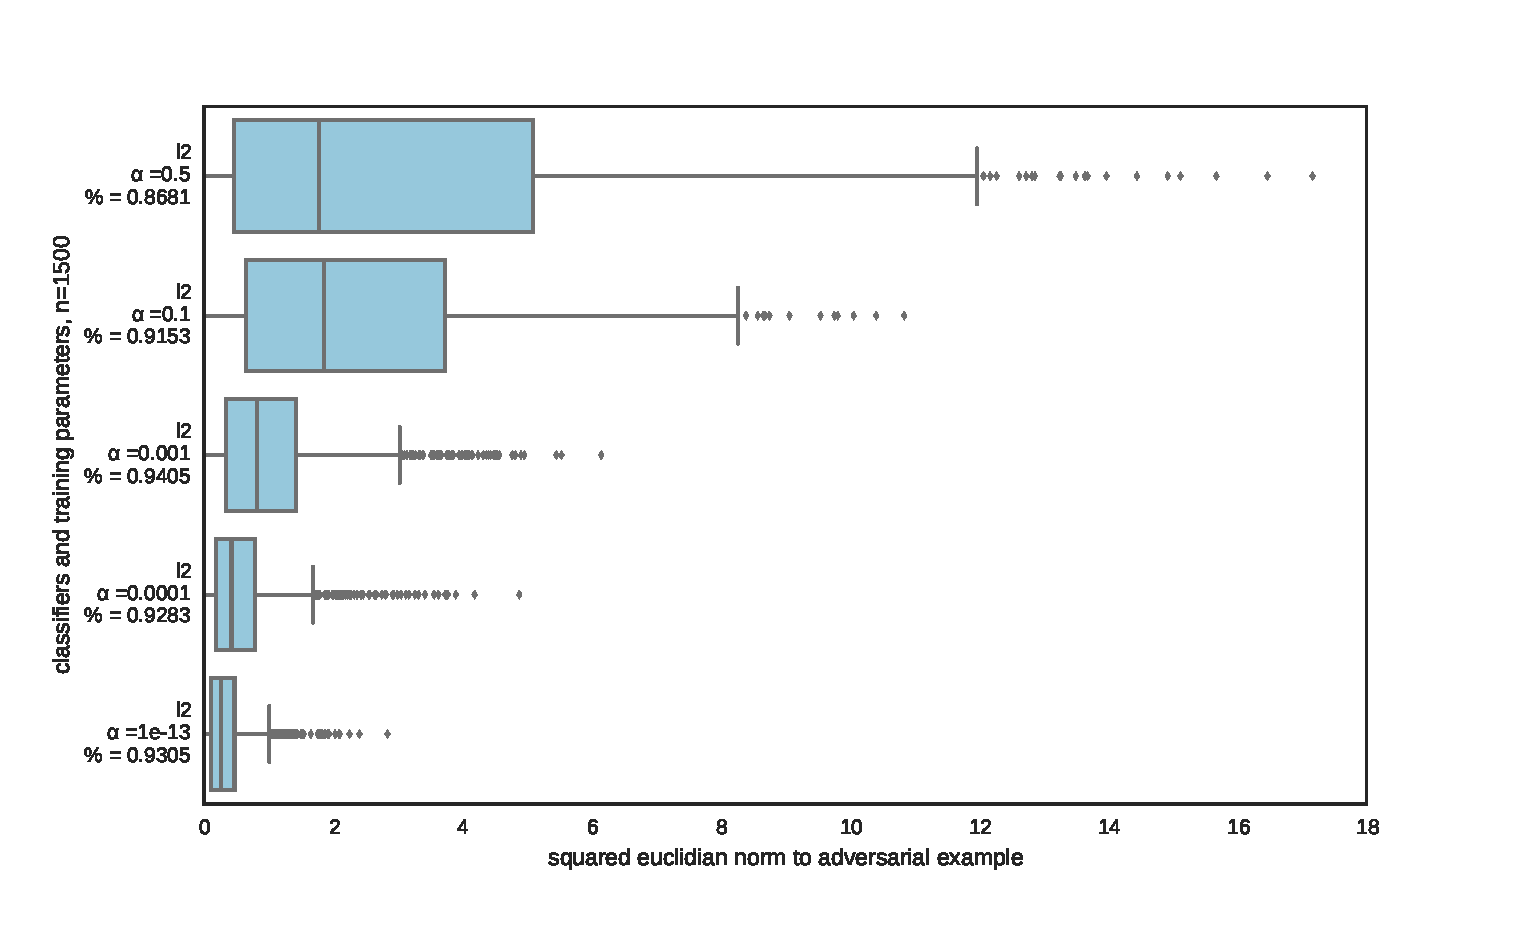
\includegraphics[scale=0.5]{figs/experiment_2_l2}
 \label{res:exp2}
 \caption{\small Improvement of robustness with regularization for the $L_2$-regularized SVM with hinge loss. The improvement in distance is very apparent as the value of $\alpha$ goes up.}
 \end{center}
\end{figure}




\subsection{class-based distribution of distances}

\begin{figure}[h!]
\begin{center}
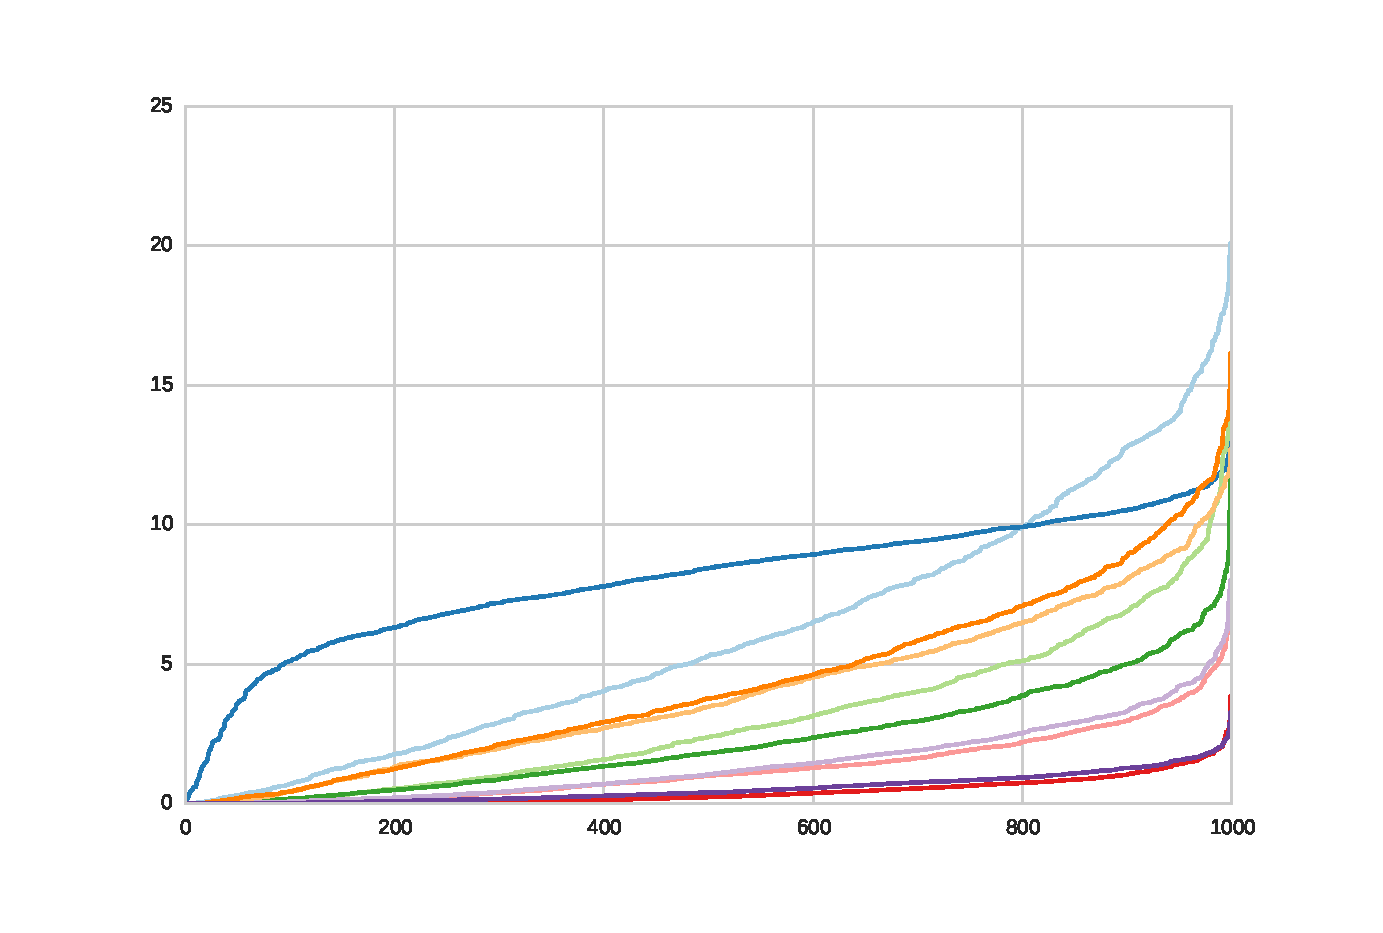
\includegraphics[scale=0.6]{figs/sup_4}
\label{exp:sup_4}
\caption{\small Comparison of the distribution of the squared norm for distorted images for each class of the
$\alpha=0.5$ $L_2$-regularized. Some classes are much
easier to generate adversarial examples from.}
\end{center}
\end{figure}

The distribution of distances for adversarial examples is quite variable and some classes are very
different for each class, and it makes sense since some of them are quite similar at the pixel level. The relation between input class and closest adversarial class was also investigated and
the results are shown in figure \ref{exp:sup_3}.

\subsection{cross-training generalization}

\begin{figure}[h!]
\begin{center}
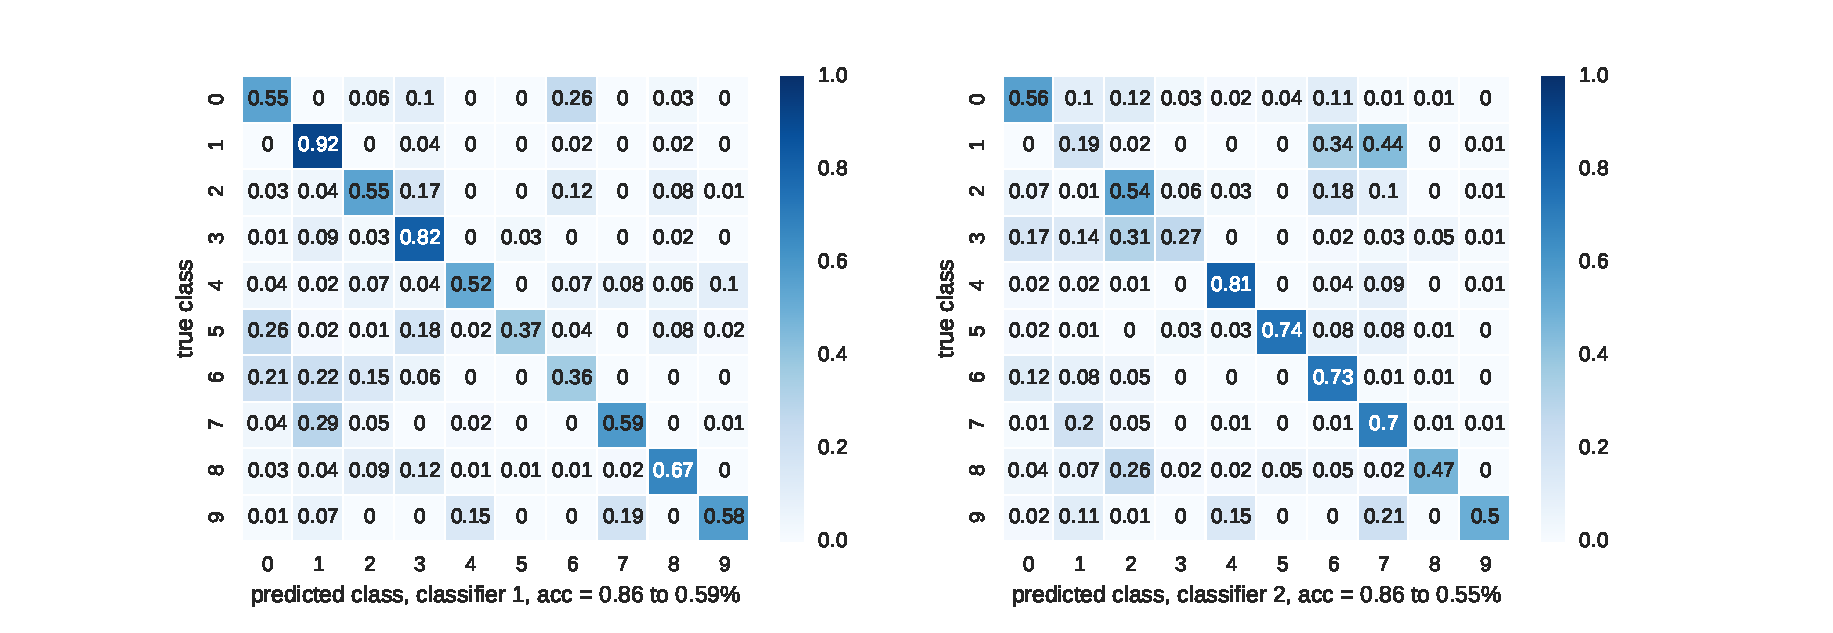
\includegraphics[scale=0.5]{figs/sup_6}
\label{exp:sup_6}
\caption{\small Class-based accuracy of cross-training generalization for two similar classifiers ($L_2$-regularized, $alpha=0.5$) trained on disjoint sets.}
\end{center}
\end{figure}

By training two classifiers on disjoint sets of the MNIST, generating adversarial examples for each (on which they have zero accuracy) and feeding them to the other classifier, we obtain this class-based accuracy (normalized on rows). Obviously, only examples that are well classified by both classifiers are pertinent to use so that limits the possible inputs. It is quite interesting to observe that they complement each other on the diagonal in that if one has a high value, the other doesn't. We are not quite sure why that is.


\null
\vfill
\newpage


\section{Discussion}

% choosing the right penalty and alpha
As expected, higher regularization penalty yields better robustness to distortion. This comes with the cost of decreasing generalization accuracy when the strength is too high. 
The $L_2$-regularized classifiers performed quite well and have a good robustness to distortion as
show in figure \ref{res:exp2}. We chose this mode of regularization with $\alpha=0.5$ for further experiments because it had the highest robustness to distortion.
The $L_1$-regularized classifiers (including the $elasticnet$) failed early, as their accuracy decreased below the fixed threshold we chose (85\% of generalization accuracy) without much impact on robustness. This is shown in figure \ref{exp:sup_2}.

% distribution of distances
We went on to observe that some input classes are more robust (especially the ones, but it makes sense since the MNIST dataset was preprocessed to straighten them). The distribution of distances for adversarial examples is presented in figure \ref{exp:sup_4}. To get a better intuition, selected examples of digits and their adversarial class counterpart are shown in figure \ref{exp:sup_5}. The smallest, median and largest required distortions were selected to give an idea of the range of distortion and the visual impact it has on the input images when using the optimization procedure. It must be remembered that the distortion can consist of adding or removing intensity by 1 bit increments and the resulting adversarial examples are valid 8-bit grayscale images. We believe the squared euclidean norm correlates well with visual impact.



% cross-training-set generalization
Finally, an experiment was done on cross-training-set generalization between two classifiers ($L_2$-regularized, $\alpha=0.5$, same as before). The 60000 MNIST dataset was split in two disjoint sets, as in \citep{szegedy_intriguing_2013}. The results are shown in figure \ref{exp:sup_6}. The accuracy
decreased by about 30\%, for both classifiers, but the interesting thing is that there is strong class bias, i.e. when one classifier correctly classified adversarial examples of its counterpart, the other one usually failed to do the same.


% conclusion and further work
In conclusion, we are quite pleased with the robustness and overall performance of the classifier. Its simplicity allowed us to devise a simple procedure to generate adversarial examples and in general, it held up quite well against distortion. 



\subsubsection*{Acknowledgments}
We would like to thank Red Bull, it gives you wings\footnote{No it doesn't. Don't sue them.}.


\bibliographystyle{plain}

\bibliography{project}


\newpage


\begin{center}
\textbf{\large Supplementary Materials}
\end{center}

\subsection{greedy optimization heuristic, the nitty–gritty details}
\label{greedy:proof}

Let $S = (o_1 , ..., o_n)$ be objects sorted in decreasing unit-value order i.e. value($o_i$)/volume($o_i$) $\geq$  value($o_{i+1}$)/volume($o_{i+1}$).

If $K$ is a choice of the first $k$ items of $S$ and $V=volume(K)$, then a knapsack of size $V$ would be optimal for the objects of $S$. This is intuitive since no other choice would have a better value/cost ratio. This is the crux of the matter for our optimization procedure.


Let $(K_1, V_1)$ and $(K_2, V_2)$, the volumes and values of two optimal knapsacks. We know that if $K_1 < K_2$ then $V_1 \leq V_2$, for we could choose the elements of $K_1$ to get an equal value or find better. This also means that given $V_1 < V_3 < V_2$ then $K_1 < K_3 < K_2$. This allows us to find bounds on $K_3$ if we know $(K_1, V_1)$ and $(K_2, V_2)$, as it must be squeezed between the two.

Although the bounds on the optimization procedure could be arbitrary big, it
is usually small for this problem, because $d$ (the threshold) is usually quite big relative
to the size of weight increments. This means tight bounds on the possible
true value of the distance.

\begin{figure}[h!]
\begin{center}
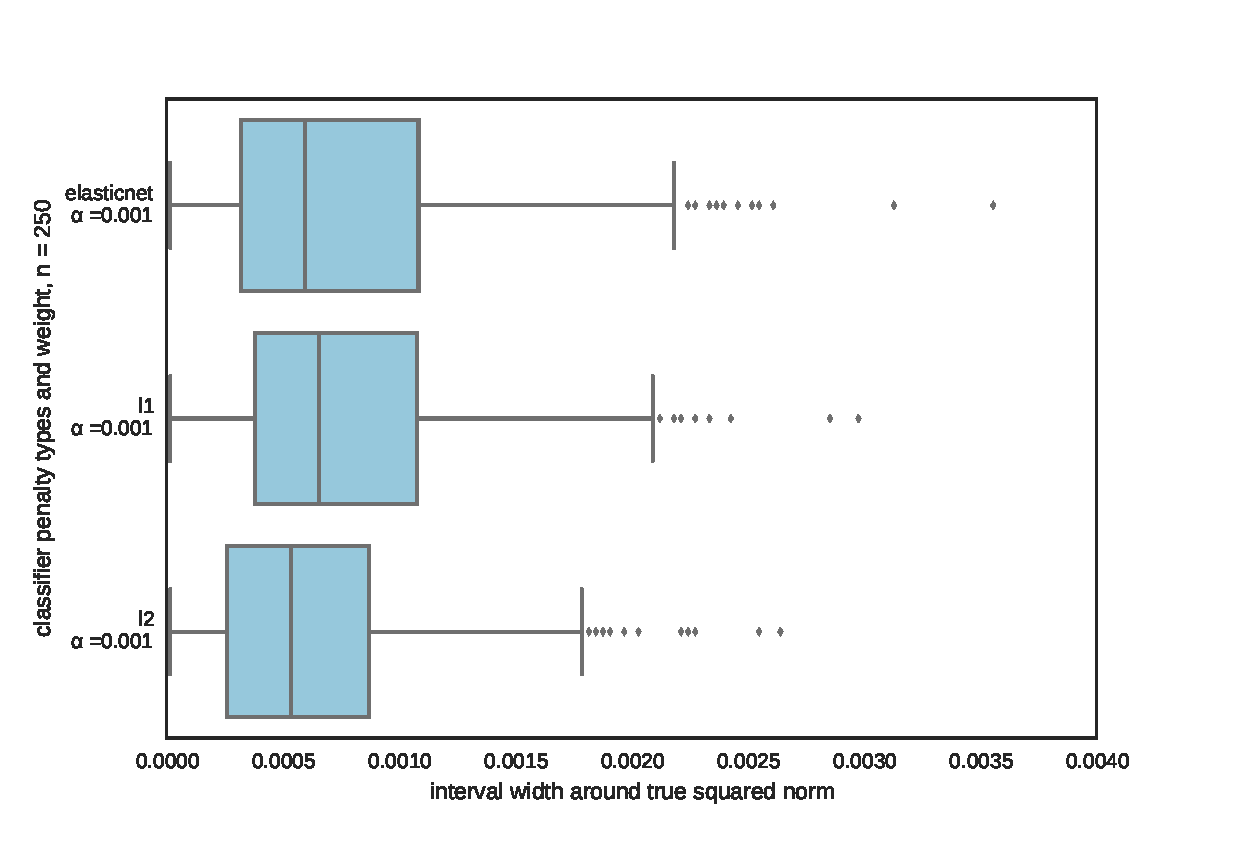
\includegraphics[scale=0.65]{figs/experiment_1}
\label{res:exp1}
\caption{\small Size of the interval on the true value of the minimal squared norm for various
                classifier on the MNIST dataset. The bound is shown to be very tight, especially considering the usual size of $d$.}
\end{center}
\end{figure}

Since the bound on the true optimal value is always very tight, the use of
the greedy optimization procedure is reasonable.


\newpage
\subsection{regularization methods and robustness}

\begin{figure}[h!]

\begin{center}
\includegraphics[scale=0.5]{figs/sup_1}
\label{exp:sup_2}
\end{center}
\caption{\small Less successful classifiers. Squared euclidian norm is relatively small in comparison to $L_2$ penalty. We see improvement as the coefficient of the penalty grows bigger.}
\end{figure}

The observation of these values prompted us to choose $L_2$-regularization for further experiments.

\null
\vfill
\newpage

\subsection{example of input and adversarial images}

\begin{figure}[h!]
\begin{center}
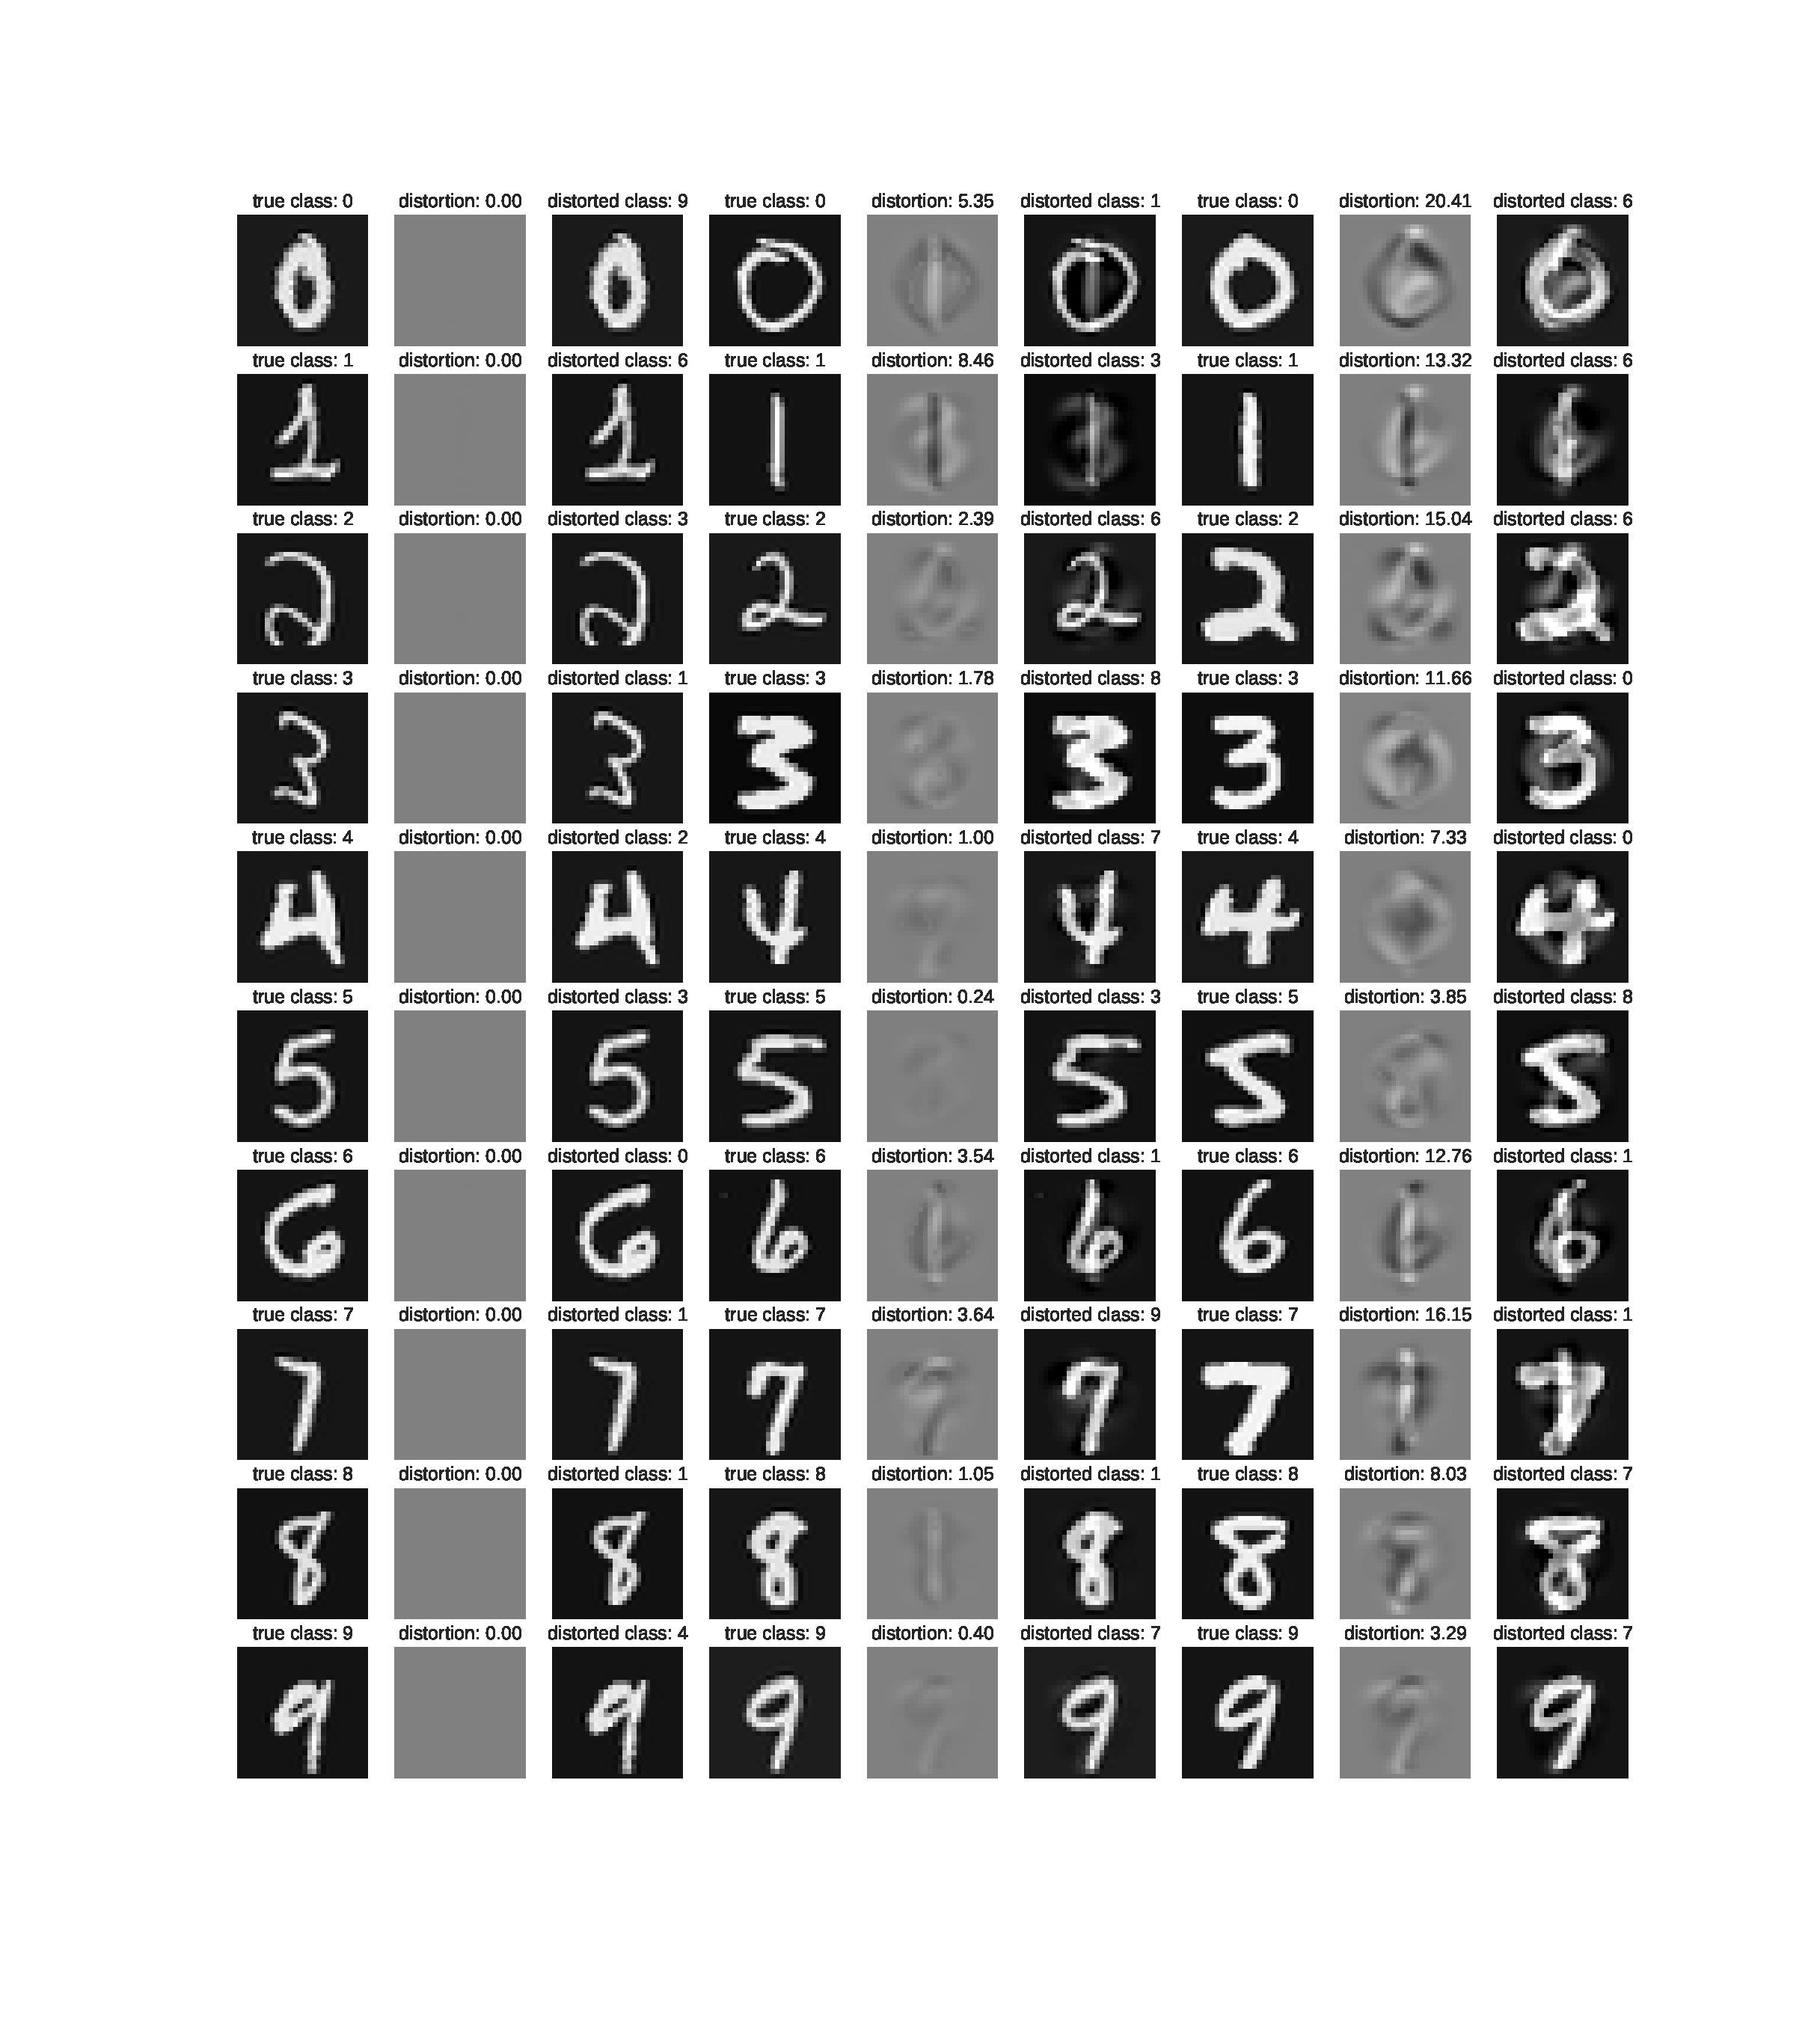
\includegraphics[scale=0.37]{figs/sup_5}
\label{exp:sup_5}
\caption{\small For each digit class, adversarial examples were generated. On each row, the 0, 50 and 100th percentiles of distances were chosen. The images are going from small to big from left to right. As can be observed, the smallest distortion is imperceptible but on the other hand, the median (50th percentile) is generally subtle. This is a good sign that the classifier is pretty robust to distortion.}
\end{center}
\end{figure}
\null
\vfill
\newpage

\subsection{relationship between input class and closest adversarial class}

\begin{figure}[h!]
\begin{center}
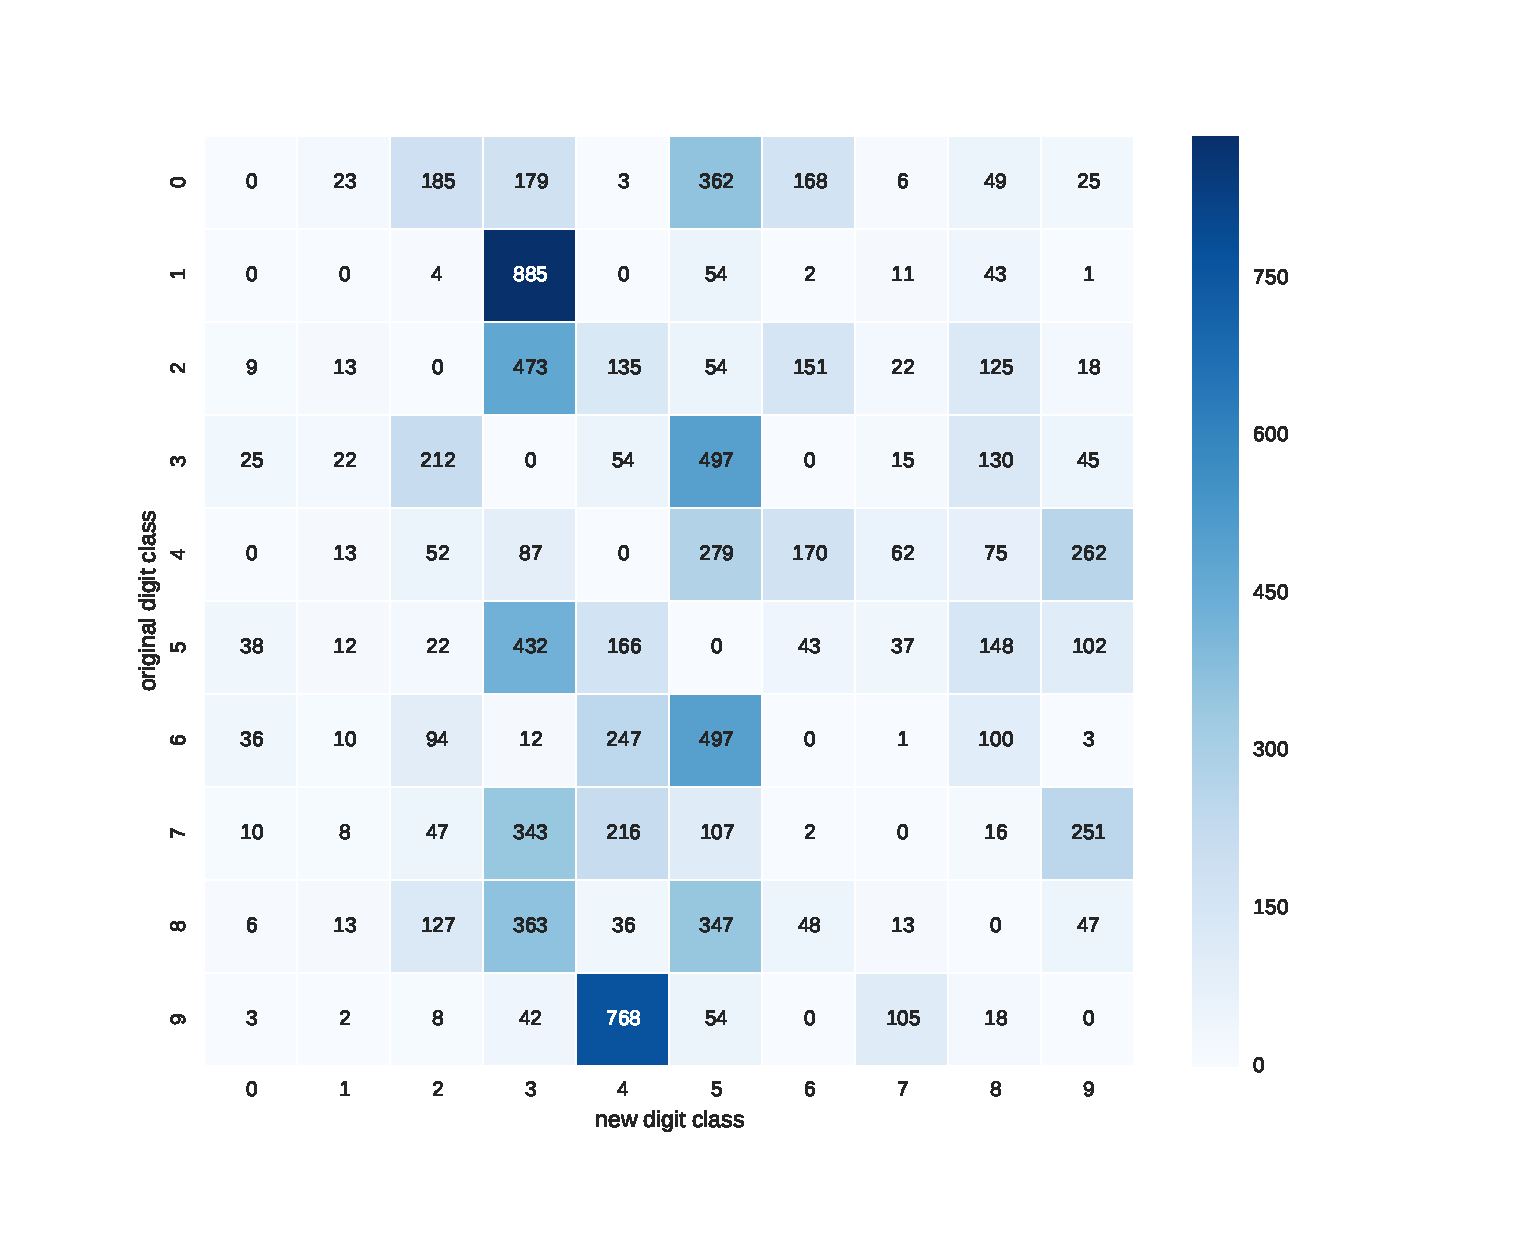
\includegraphics[scale=0.6]{figs/sup_3}
\label{exp:sup_3}
\caption{\small Classes of the adversarial examples generated.
For each original class, 1000 images were chosen (rows sum to 1000). We can see quite a strong bias to some classes, especially for class 1 and 9.}
\end{center}
\end{figure}

\null
\vfill
\newpage






\end{document}


